% This file was created by matlab2tikz.
%
%The latest updates can be retrieved from
%  http://www.mathworks.com/matlabcentral/fileexchange/22022-matlab2tikz-matlab2tikz
%where you can also make suggestions and rate matlab2tikz.
%
\definecolor{mycolor1}{rgb}{0.49412,0.18431,0.55686}%
\definecolor{mycolor2}{rgb}{1.00000,0.41176,0.16078}%
%
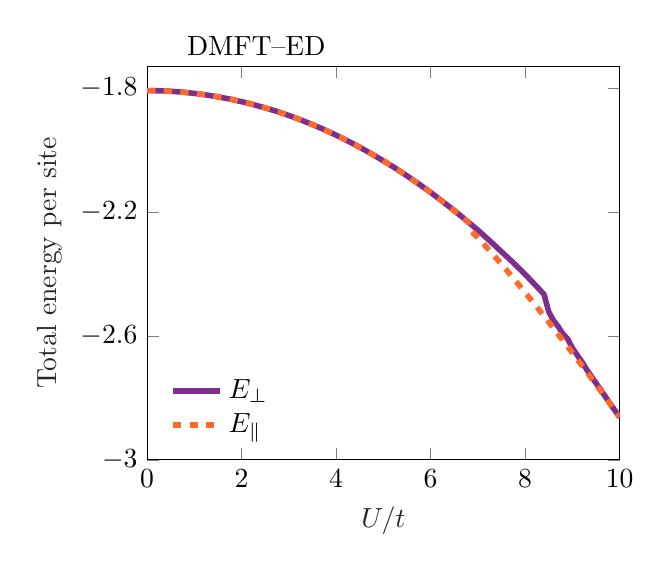
\begin{tikzpicture}

\begin{axis}[%
width=6cm,
height=5cm,
at={(0cm,0cm)},
scale only axis,
xmin=0,
xmax=10,
xlabel style={font=\color{white!15!black}},
xlabel={$U/t$},
ymin=-3,
ymax=-1.73,
ytick={-3,-2.6,-2.2,-1.8},
ylabel style={font=\color{white!15!black}},
ylabel={Total energy per site},
axis background/.style={fill=white},
legend style={at={(0.03,0.03)}, anchor=south west, legend cell align=left, align=left, fill=none, draw=none}
]
\addplot [color=mycolor1, line width=2.0pt]
  table[row sep=crcr]{%
0	-1.808924136\\
0.25	-1.809478441\\
0.5	-1.811149576\\
0.75	-1.813937471\\
1	-1.817851655\\
1.25	-1.822893129\\
1.5	-1.829051734\\
1.75	-1.836244458\\
2	-1.844655547\\
2.25	-1.854195896\\
2.5	-1.864848693\\
2.75	-1.876246734\\
3	-1.88918081\\
3.25	-1.903285582\\
3.5	-1.918560433\\
3.75	-1.935032745\\
4	-1.952713328\\
4.25	-1.971619432\\
4.5	-1.991555324\\
4.75	-2.012929432\\
5	-2.035457937\\
5.25	-2.058808198\\
5.5	-2.083784684\\
5.75	-2.110149044\\
6	-2.137154072\\
6.25	-2.166286327\\
6.5	-2.195608428\\
6.75	-2.22709923\\
7	-2.25882618\\
7.25	-2.293228913\\
7.5	-2.328536192\\
7.75	-2.364215635\\
8	-2.401539097\\
8.25	-2.441646876\\
8.3	-2.449684048\\
8.4	-2.466310382\\
8.5	-2.522448093\\
8.6	-2.550136378\\
8.7	-2.570136427\\
8.8	-2.593980148\\
8.9	-2.609876089\\
9	-2.639432545\\
9.1	-2.661537072\\
9.2	-2.683452941\\
9.3	-2.707815447\\
9.4	-2.730243038\\
9.5	-2.752408766\\
9.6	-2.774077316\\
9.7	-2.796405298\\
9.8	-2.818931809\\
9.9	-2.84055057\\
10	-2.863419743\\
};
\addlegendentry{$E_\perp$}

\addplot [color=mycolor2, dashed, line width=2.0pt]
  table[row sep=crcr]{%
0	-1.808924136\\
0.1	-1.809012633\\
0.2	-1.80927993\\
0.3	-1.809724646\\
0.4	-1.810347414\\
0.5	-1.811148013\\
0.6	-1.812126831\\
0.7	-1.813283796\\
0.8	-1.814619013\\
0.9	-1.816132545\\
1	-1.81782444\\
1.1	-1.819695118\\
1.2	-1.821745183\\
1.3	-1.82397425\\
1.4	-1.826381633\\
1.5	-1.828969857\\
1.6	-1.831728692\\
1.7	-1.83467677\\
1.8	-1.837799082\\
1.9	-1.841107346\\
2	-1.844595359\\
2.1	-1.848254395\\
2.2	-1.852104642\\
2.3	-1.856136236\\
2.4	-1.860354176\\
2.5	-1.864752208\\
2.6	-1.869257968\\
2.7	-1.87402614\\
2.8	-1.878977189\\
2.9	-1.884112579\\
3	-1.889433508\\
3.1	-1.894940561\\
3.2	-1.900634076\\
3.3	-1.906514308\\
3.4	-1.912581475\\
3.5	-1.918835824\\
3.6	-1.925277744\\
3.7	-1.931907867\\
3.8	-1.938727054\\
3.9	-1.945736271\\
4	-1.952936449\\
4.1	-1.960328441\\
4.2	-1.967913029\\
4.3	-1.975690969\\
4.4	-1.983663005\\
4.5	-1.991829898\\
4.6	-2.000192413\\
4.7	-2.008751334\\
4.8	-2.017507458\\
4.9	-2.026461597\\
5	-2.035624426\\
5.1	-2.044952221\\
5.2	-2.054477178\\
5.3	-2.06422158\\
5.4	-2.074115762\\
5.5	-2.084243211\\
5.6	-2.094534447\\
5.7	-2.105072301\\
5.8	-2.115834947\\
5.9	-2.126791565\\
6	-2.137966448\\
6.1	-2.149342173\\
6.2	-2.160929849\\
6.3	-2.172728017\\
6.4	-2.184738284\\
6.5	-2.196947161\\
6.6	-2.209361283\\
6.7	-2.221704237\\
6.8	-2.234060095\\
6.81	-2.250969446\\
6.82	-2.255423674\\
6.83	-2.256951827\\
6.84	-2.258621179\\
6.85	-2.260276753\\
6.86	-2.261800925\\
6.87	-2.263462778\\
6.88	-2.265013364\\
6.89	-2.266635577\\
6.9	-2.268246734\\
7	-2.283675823\\
7.1	-2.300327992\\
7.2	-2.317123659\\
7.3	-2.334214642\\
7.4	-2.351528503\\
7.5	-2.369075044\\
7.6	-2.386868463\\
7.7	-2.404856687\\
7.8	-2.423091712\\
7.9	-2.441489537\\
8	-2.460083731\\
8.1	-2.478914857\\
8.2	-2.497766571\\
8.3	-2.516954677\\
8.4	-2.536162087\\
8.5	-2.55560576\\
8.6	-2.575102434\\
8.7	-2.594851614\\
8.8	-2.614636481\\
8.9	-2.634594411\\
9	-2.654722881\\
9.1	-2.674887929\\
9.2	-2.695162154\\
9.3	-2.715786261\\
9.4	-2.736227728\\
9.5	-2.756902955\\
9.6	-2.777771029\\
9.7	-2.798696121\\
9.8	-2.819702455\\
9.9	-2.840743591\\
10	-2.861912101\\
};
\addlegendentry{$E_\parallel$}

\end{axis}

\begin{axis}[%
width=6.135cm,
height=4.908cm,
at={(-0.798cm,-0.54cm)},
scale only axis,
xmin=0,
xmax=1,
ymin=0,
ymax=1,
axis line style={draw=none},
ticks=none,
axis x line*=bottom,
axis y line*=left
]
\end{axis}

\node[above left]
at (current bounding box.north) {DMFT--ED};

\end{tikzpicture}%